\documentclass[conference]{IEEEtran}
\IEEEoverridecommandlockouts
% The preceding line is only needed to identify funding in the first footnote. If that is unneeded, please comment it out.
\usepackage{cite}
\usepackage{amsmath,amssymb,amsfonts}
\usepackage{algorithmic}
\usepackage{graphicx}
\usepackage{textcomp}
\usepackage{xcolor}

% Pacotes adicionados para suporte à língua portuguesa
\usepackage[utf8]{inputenc}
\usepackage[T1]{fontenc}
\usepackage[portuguese]{babel}

\def\BibTeX{{\rm B\kern-.05em{\sc i\kern-.025em b}\kern-.08em
    T\kern-.1667em\lower.7ex\hbox{E}\kern-.125emX}}
\begin{document}

\title{Spillover Effect em jogos indies: Análise Estatística\\
%{\footnotesize \textsuperscript{*}Nota: Subtítulos não são capturados no Xplore e não devem ser usados}
\thanks{Identifique a agência de financiamento aqui. Se não houver, exclua isto.}
}

\author{\IEEEauthorblockN{1\textsuperscript{st} Marcus Cavalcante - 160135974}
\IEEEauthorblockA{\textit{Departamento de Ciência da Computação} \\
Ciência da Computação \\
\textit{Universidade de Brasília}\\
Brasília - DF, Brasil \\
mv.balbc@gmail.com}
\and
\IEEEauthorblockN{2\textsuperscript{nd} João Zago}
\IEEEauthorblockA{\textit{departamento / curso} \\
\textit{nome da instituição}\\
Cidade, País \\
email ou ORCID}
\and
\IEEEauthorblockN{3\textsuperscript{} Gustavo Macedo}
\IEEEauthorblockA{\textit{departamento / curso} \\
\textit{nome da instituição}\\
Cidade, País \\
email ou ORCID}
% Adicione mais blocos de autores conforme necessário (3rd, 4th, etc.)
}

\maketitle

\begin{abstract}
Este resumo deve conter uma síntese de toda a sua pesquisa. 
Indique o contexto do problema, qual base de dados foi utilizada, 
o objetivo principal de se realizar uma análise estatística 
descritiva e os principais resultados e insights encontrados. 
O resumo deve ser conciso e permitir que o leitor entenda 
rapidamente a essência do trabalho.
\end{abstract}

\begin{IEEEkeywords}
análise estatística, análise descritiva, banco de dados, \textit{data science}.
\end{IEEEkeywords}

\section{Introdução}
O mercado de jogos independentes (indie) tem crescido nas últimas décadas, 
tornando-se um dos pilares de inovação da indústria de entretenimento digital. 
Com o aumento da competitividade, o comportamento dos estúdios no que concerne 
à criação de continuações e franquias tornou-se um fenômeno relevante de estudo. 
Neste contexto, o \textit{spillover effect} (ou Efeito Halo) é um conceito que 
descreve como a percepção positiva ou o sucesso de um produto pode transbordar 
para outros da mesma marca. 
Na indústria de jogos, isso se traduz no aumento do interesse em títulos 
anteriores de um estúdio após o lançamento de uma sequência bem-sucedida.

Este artigo realiza uma análise estatística descritiva focada em explorar o 
impacto das continuações no mercado indie. Nossa pesquisa busca responder a seis 
questões principais utilizando dados reais de mercado:

\begin{itemize}
    \item \textbf{1º O "Efeito Halo" é real nos jogos indie?} 
    Jogos originais de estúdios que lançaram sequências possuem um volume 
    de vendas acumuladas significativamente maior do que jogos únicos de 
    estúdios que nunca tiveram sequências?
    \item \textbf{2º Qual a recepção crítica?} 
    A nota média das sequências é maior, menor ou igual à dos jogos originais indie?
\end{itemize}   

O restante deste artigo detalha a metodologia de obtenção e pré-processamento 
dos dados na Seção II e apresenta os resultados quantitativos obtidos 
acompanhados de recursos visuais na Seção III.

\section{Metodologia}
A presente seção descreve a origem dos dados e os procedimentos metodológicos 
adotados para a análise descritiva, abordando o tratamento necessário para 
estruturar as categorias de interesse.

\subsection{Descrição da Base de Dados}
Os dados foram extraídos do dataset "Steam Games Dataset" disponibilizado 
publicamente no Kaggle, que compila metadados e estatísticas de milhares de 
jogos listados na plataforma de distribuição digital Steam. 
O arquivo original (\texttt{steam\_games.csv}) contém mais de 
120.000 instâncias e quase 40 atributos. Para a finalidade deste estudo, 
aplicou-se um recorte focado exclusivamente no mercado indie, 
filtrando apenas as entradas em que a tag "Indie" estivesse presente no 
campo de gêneros. Adicionalmente, limitamos a amostra a jogos lançados a 
partir do ano de 2016 e com preço superior a \$1 dólar, com a finalidade 
de expurgar da análise jogos de qualidade duvidosa (\textit{shovelware}) 
ou produtos abandonados e gratuitos que não representam o mercado 
competitivo real. O escopo final da nossa análise resultou em 
50.464 jogos independentes.

\subsection{Dicionário de Variáveis}
As variáveis utilizadas para testar o fenômeno do Efeito Halo e a 
percepção crítica estão descritas na Tabela \ref{tab_variaveis}. 

\begin{table}[htbp]
\caption{Principais Variáveis Analisadas}
\begin{center}
\begin{tabular}{|c|c|p{4cm}|}
\hline
\textbf{Variável} & \textbf{Tipo} & \textbf{Descrição} \\
\hline
\textit{Owners} & Numérica Contínua & Proxy de vendas acumuladas. 
É calculado tirando a média da faixa estimada fornecida pela Steam 
(ex: a faixa "0 - 20000" equivale a 10000). \\
\hline
\textit{Score} & Numérica Contínua & Nota do jogo em formato de proporção, 
calculada através da razão de interações positivas pelo número total de 
interações (Positivas + Negativas). \\
\hline
\textit{Category} & Qualitativa Nominal & Classificação do título gerada 
pelas heurísticas textuais (Original, Sequência, ou Jogo Único). \\
\hline
\end{tabular}
\label{tab_variaveis}
\end{center}
\end{table}

\subsection{Pré-processamento e Limpeza dos Dados}
A separação das categorias (Jogos Originais e Sequências) constituiu o 
maior desafio de tratamento dos dados, pois o \textit{dataset} do 
Kaggle não inclui uma coluna oficial relacionando as franquias 
(\textit{Franchise ID}). Para contornar essa limitação, 
aplicou-se uma heurística baseada no agrupamento por estúdio desenvolvedor. 
Estúdios com apenas um jogo publicado foram direcionados 
automaticamente à categoria "Jogo Único". 
Para desenvolvedoras com múltiplos títulos, os nomes foram normalizados 
e submetidos a expressões regulares (\textit{regex}) 
preparadas para detectar marcadores numéricos e subtítulos 
clássicos de sequências (ex: "2", "II", "Part", "Return"). 
Jogos detectados foram classificados como "Sequência", 
e os demais títulos do mesmo desenvolvedor foram enquadrados 
como "Original". Jogos com notas não computáveis (zero reviews) 
foram desconsiderados do cálculo de notas, e valores nulos na 
categoria "Preço" foram descartados durante o pré-processamento.

\section{Resultados: Análise Estatística Descritiva}
Esta seção apresenta os resultados obtidos a partir do processamento e 
categorização dos dados do mercado de jogos independentes na Steam, 
respondendo às perguntas propostas com base nas estatísticas extraídas.

\subsection{O Efeito Halo e as Vendas Acumuladas}
Para avaliar a existência de um Efeito Halo, comparou-se a métrica de "donos estimados" 
(\textit{estimated owners}), que atua como \textit{proxy} para as vendas acumuladas. 

A média de donos para jogos \textbf{originais que possuem sequências} 
foi de \textbf{52.258}, enquanto a média para 
\textbf{jogos únicos (de estúdios sem sequências)} foi inferior, 
contabilizando \textbf{51.177}. Apesar da mediana permanecer 
estabilizada na faixa de 10.000 cópias em ambos os grupos devido 
às faixas de aproximação fornecidas pela plataforma (ex: "0 - 20000"), 
a diferença na média ainda indica uma presença do \textit{spillover effect}, 
mesmo com o filtro de jogos mais recentes (a partir de 2016) e 
precificados (acima de \$1). Em resumo, títulos que dão origem a 
franquias demonstram capacidade de atrair um público acumulado superior, 
indicando um provável tráfego direcionado das sequências de volta aos jogos primordiais.

\begin{figure}[htbp]
\centerline{
\includegraphics[width=\linewidth]{plot_owners.png}}
\caption{Comparativo da média de vendas acumuladas (Owners) entre jogos 
originais de franquias e jogos únicos.}
\label{fig_owners}
\end{figure}

\subsection{Avaliação e Engajamento Crítico}
A segunda parte da nossa investigação tratou da qualidade percebida e 
engajamento do público medido pela nota média do jogo 
(calculada pela proporção de avaliações positivas sobre o total de interações).

Ao observar as pontuações, a nota mediana das \textbf{sequências} foi de 
\textbf{85.73\%} (com média de 80.51\%). Por outro lado, a nota mediana dos 
\textbf{jogos originais} do nosso conjunto de dados ficou em 
\textbf{82.99\%} (com média de 77.04\%).  

Esses resultados indicam de forma evidente que as sequências, 
no mercado indie, tendem a receber pontuações e percentuais de aprovação 
superiores aos originais. Isso pode ocorrer porque continuações 
se beneficiam do aprendizado do estúdio, capitalizam sobre mecânicas 
de jogo já consagradas pelo título de estreia, 
e muitas vezes engajam uma base de fãs mais 
direcionada e menos propensa a avaliações negativas casuais.

\begin{figure}[htbp]
\centerline{
\includegraphics[width=\linewidth]{plot_scores.png}}
\caption{Comparativo da nota média e de aprovação das Sequências versus 
os Jogos Originais que lhes deram origem.}
\label{fig_scores}
\end{figure}

A Figura \ref{fig_boxplot_scores} atesta de forma gráfica a variação das 
pontuações. Os \textit{boxplots} deixam claro que as sequências 
operam com uma margem interquartil em uma faixa de aprovação 
visivelmente superior, além da mediana estar estabelecida 
alguns degraus acima da linha central do catálogo dos originais.

\begin{figure}[htbp]
\centerline{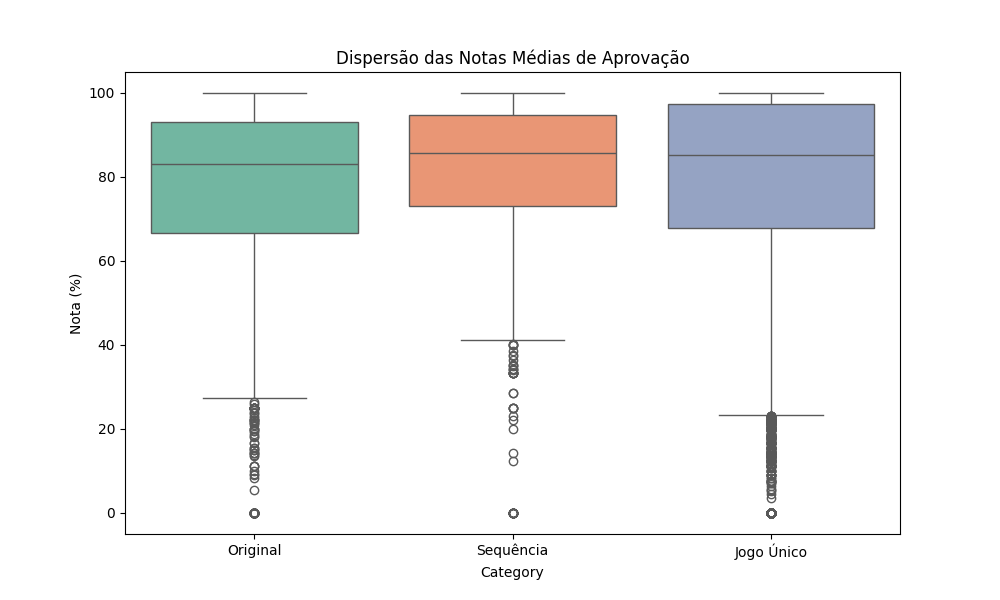
\includegraphics[width=\linewidth]{boxplot_scores.png}}
\caption{Dispersão estatística (Boxplot) das Notas Médias de Aprovação.}
\label{fig_boxplot_scores}
\end{figure}

\section{Discussão dos Resultados}
Os \textit{insights} recolhidos demonstram que, ao menos no nicho de mercado 
Indie após 2016 e para títulos efetivamente comercializados (> \$1), 
as continuações jogam um papel estatístico claro. 

O lançamento de uma continuação serve não apenas como uma nova via de 
capitalização, mas atua quase que como um instrumento massivo de 
\textit{marketing} para os títulos do passado, 
efetivando o \textit{Spillover Effect}. 

Do ponto de vista qualitativo, o padrão é que continuações são, 
em geral, mais bem avaliadas do que suas fontes originárias. 
Pode-se conjecturar que uma sequência beneficia-se do feedback 
inicial do público da franquia, garantindo correções em escopo 
de \textit{design}, ao passo que desfruta da indulgência e 
maior engajamento de uma comunidade de fãs já dedicada e 
menos propensa a avaliações negativas aleatórias.

\section{Conclusão e Trabalhos Futuros}
Esta pesquisa realizou uma análise quantitativa descritiva 
focada em examinar as consequências no engajamento e nas vendas ao se 
estabelecer continuações na indústria de jogos independentes. 
Constatou-se não só a prevalência do Efeito Halo sobre o catálogo 
pretérito de estúdios prolíficos, como também que sequências 
carregam margens estatisticamente superiores de aprovação da comunidade. 

No entanto, é vital destacar as limitações metodológicas: o dataset 
fornecido funciona como uma fotografia estática do mercado, 
impedindo observações puras de séries temporais. Adicionalmente, 
a ausência de uma catalogação oficial por \textit{Franchise ID} 
impôs a utilização de uma heurística por Expressões Regulares de 
títulos que inerentemente insere a margem para erros e \textit{outliers} 
não triviais à análise.

Para trabalhos futuros, recomenda-se integrar a mineração de dados com 
chamadas de rede em APIs oficias (como SteamDB ou SteamSpy) para colher 
explícitamente as associações das franquias, garantindo 100\% de confiança 
à categoria. Ademais, seria benéfico empregar testes de hipótese 
inferenciais (Testes-T ou Mann-Whitney) para sedimentar de vez a 
força estatística das médias extraídas neste ensaio empírico.

\section*{Agradecimentos}
Gostaríamos de agradecer o constante incentivo da Universidade de 
Brasília e aos responsáveis pela curadoria de dados da Steam, cujo 
ecossistema possibilita essa democratização de dados científicos na 
área de computação e negócios.


\begin{thebibliography}{00}
\bibitem{b2} Kaggle, ``Steam Games Dataset'', Disponível em: 
\texttt{https://www.kaggle.com/datasets/fronkongames\\/steam-games-dataset}. Acesso em: 1 jun. 2026.
\bibitem{b3} W. McKinney, ``Data Structures for Statistical Computing in Python,'' nas \textit{Proc. of the 9th Python in Science Conference}, pp. 51--56, 2010.
\end{thebibliography}

\end{document}
